\section{Колірні моделі та простори}

Оскільки цифрова електроніка оперує лише дискретною математикою, то над вченими 20 століття постала проблема представлення кольорів у ЕОМ. Основна ідея представлення кольорів прийшла з науки біології та експериментальним шляхом було доведено, що людина є трихроматом \cite{ColorSeing}. Сітчатка ока трихроматів має 3 види рецепторів, що називаються ковбочками, які відповідають за колірний зір. Кожна з цих ковбочок має як параметр деяку довжину хвилі, на яку вона дає максимальний зворотній сигнал.

\subsection{RGB}
RGB (скорочено від англ. Red, Green, Blue — червоний, зелений, синій) — адитивна колірна модель, що описує спосіб синтезу кольору, за якою червоне, зелене та синє світло накладаються разом, змішуючись у різноманітні кольори. Широко застосовується в техніці, що відтворює зображення за допомогою випромінення світла.

У даній моделі колір кодуєтся градаціями складових каналів (Red, Green, Blue). Тому за збільшення величини градації котрогось каналу — зростає його інтенсивність під час синтезу.

Кількість градацій кожного каналу залежить від розрядності бітового значення RGB. Зазвичай використовують 24-бітну модель, у котрій визначається по 8 біт на кожен канал, і тому кількість градацій дорівнює 256, що дозволяє закодувати 2563 = 16 777 216  кольорів.

\begin{figure}[H]
	\centering
	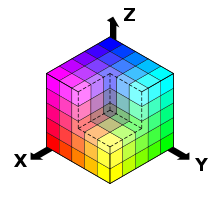
\includegraphics[width=0.7\linewidth]{theory/img/rgb_representation}
	\caption{Тривимірне представлення моделі RGB}
\end{figure}

Колірна модель RGB призначена сприймати, представляти та відображати зображення в електронних системах, таких як телебачення та комп'ютери, хоча її також застосовували у традиційній фотографії. Вже до електронного віку, модель RGB мала за собою серйозну теорію, засновану на сприйнятті кольорів людиною.

Типово приладами із RGB-входом є кольоровий телевізор і відеокамера, сканер і цифровий фотоапарат.

\begin{figure}[H]
	\centering
	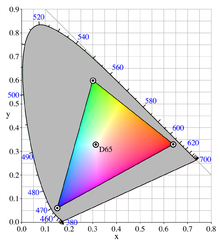
\includegraphics[width=0.7\linewidth]{theory/img/rgb_limitations}
	\caption{Обмеженість моделі по можливості передачі кольору}
\end{figure}

Переваги моделі:
\begin{enumerate}
	\item Апаратна близкість із монітором, сканером, проектором, іншими пристроями;
	\item Велика кольорова гама, близька до можливостей людського зору;
	\item Доступність багатьох функцій обробки зображення (фільтрів) у програмах растрової графіки;
	\item Невеликий (порівняно до моделі CMYK) обсяг, проте ширший спектр кольорів.
\end{enumerate}
\bigbreak
Недоліки:
\begin{enumerate}
	\item Обмеженість моделі;
	\item Немає явного відділення люмінантної компоненти - для аналізу яскравості пікселя потрібно робити додаткові перетворення.
\end{enumerate}

\subsection{HSV,HSL}
HSB — колірна модель, що використовується тільки для оформлення векторних і текстових об'єктів документа. Описує колірний простір, заснований на трьох характеристиках кольору: колірному тоні (Hue), насиченості (Saturation) і яскравості (Brightness).

\begin{itemize}
	\item Hue — колірний тон, (наприклад, червоний, зелений або синьо-блакитний). Варіюється в межах 0-360°, але іноді приводиться до діапазону 0-100 або 0-1. У Windows весь колірний спектр ділиться на 240 відтінків (що можна спостерігати в редакторі палітри MS Paint), тобто тут «Hue» зводиться до діапазону 0-240 (відтінок 240 відсутній, оскільки він дублював би 0).

	\item Saturation — насиченість. Варіюється в межах 0-100 або 0-1. Чим більший цей параметр, тим «чистіший» колір, тому цей параметр іноді називають чистотою кольору. А чим ближчий цей параметр до нуля, тим ближчий колір до нейтрального сірого.
	
	\item Value (значення кольору) або Brightness — яскравість. Також задається в межах 0-100 або 0-1.
\end{itemize}

Модель була створена Елві Реєм Смітом, одним із засновників Pixar, в 1978 році. Вона є нелінійним перетворенням моделі RGB.

Колір, представлений в HSV, залежить від пристрою, на який він буде виведений, так як HSV — перетворення моделі RGB, яка теж залежить від пристрою. Для отримання коду кольору, не залежного від пристрою, використовується модель Lab.

\subsection{Lab}

\subsection{YCrCb}
